\documentclass[xcolor={usenames,dvipsnames}]{beamer}

\usepackage[utf8]{inputenc}
\usepackage[english]{babel}

\usepackage{graphicx}
\usepackage{amsmath}
\usepackage{amssymb}
\usepackage{amsthm}
\usepackage{array}

\usepackage{alltt}

\addtocounter{footnote}{1}
\setcounter{tocdepth}{5}
\setcounter{secnumdepth}{5}
\renewcommand{\floatpagefraction}{0.75}

%Information to be included in the title page:
\title{Recap: Concurrency Control}
\author{Alexander Christensen}
\institute{Department of Computer Science \\ University of Copenhagen}
\date{2021}

%% Reference an equation, a figure, or a section

%% \secref{label} - make a reference to a section
\newcommand{\secref}[1]{Section~\ref{#1}}

%% \eqref{reference} - make a reference to an equation
%%\newcommand{\eqref}[1]{(\ref{#1})}

%% \figref{reference} - make a reference to an figure
\newcommand{\figref}[1]{Figure~\ref{#1}}

\newcommand{\basetop}[1]{\vtop{\vskip-1ex\hbox{#1}}}
\newcommand{\source}[1]{\let\thefootnote\relax\footnotetext{\scriptsize\textcolor{kugray1}{Source: #1}}}

%\bibliographystyle{longalpha}
%\bibliography{refs}

%% -*- Mode: latex -*-

%% Macros defined during a long time and used much
% plus - a plus sign
\newcommand{\plus}{+}

% minus - a minus having the same width as a plus
\newlength{\minuswidth}
\settowidth{\minuswidth}{+}
\newlength{\minusheight}
\settoheight{\minusheight}{+}
\newcommand{\minus}{\rule[0.5\minusheight]{\minuswidth}{0.5pt}}

% The basis vector standard
%\renewcommand{\vec}[1]{\boldsymbol{#1}}
\newcommand{\grad}{\operatorname{\nabla}}
\newcommand{\curl}{\operatorname{\text{curl}}}
\newcommand{\divergence}{\operatorname{\text{div}}}
\newcommand{\vecop}{\operatorname{\text{vec}}}
\newcommand{\diag}{\operatorname{\text{diag}}}
\renewcommand{\Re}{\mathbb{R}}
\newcommand{\Co}{\mathbb{C}}
\newcommand{\In}{\mathbb{Z}}
\newcommand{\sign}{\operatorname{sgn}}
%\newcommand{\trace}{\operatorname{Tr}}
\newcommand{\arctantwo}{\ensuremath{\arctan\!2}}
%\newcommand{\mat}[1]{\ensuremath{\boldsymbol{#1} }}
\newcommand{\I}{\mat{1}}
\newcommand{\crossmat}[1]{\ensuremath{\boldsymbol{#1}^{\times} }}
\newcommand{\jacobian}[1]{\ensuremath{\boldsymbol{\mathit{#1}} }}
\newcommand{\set}[1]{\ensuremath{ \boldsymbol{#1} }}
\newcommand{\func}[1]{{\bf{#1}}}
\newcommand{\enorm}[1]{\ensuremath{\left\| #1 \right\|_{_2}}}
%\newcommand{\norm}[1]{\ensuremath{\left\| #1 \right\|}}
\newcommand{\bdet}[1]{\ensuremath{\left| #1 \right|}}
\newcommand{\abs}[1]{\ensuremath{\left| #1 \right|}}
\newcommand{\rtm}{$^{\textrm{®}}$}


\newcommand{\kenny}[1]{ #1 }
\newcommand{\henrik}[1]{ #1 }


%% \maya - the maya signature
\newcommand{\maya}{$ \texttt{Maya}^{\text{\texttrademark}} $}

%% \fat{symbol} - make this symbol fat
\newcommand{\fat}[1]{\mathit{\mathbf{#1}}}
%% \newcommand{\fat}[1]{\hbox{\boldmath $ #1 $}}

%% \vec{symbol} - Vector
%% \renewcommand{\vec}[1]{\mathbf{#1}}
\renewcommand{\vec}[1]{\fat{#1}}

%% \mat{symbol} - Matrix
%%\newcommand{\mat}[1]{\ensuremath{\boldsymbol{#1} }}
\newcommand{\mat}[1]{\fat{#1}}

%% \ezero,...,\ethree - the spin matrices
\newcommand{\ezero}{\begin{bmatrix} 1 & 0 \\  0 &  1 \end{bmatrix}}
\newcommand{\eone}{\begin{bmatrix} i & 0 \\  0 & -i \end{bmatrix}}
\newcommand{\etwo}{\begin{bmatrix} 0 & 1 \\ -1 &  0 \end{bmatrix}}
\newcommand{\ethree}{\begin{bmatrix} 0 & i \\  i &  0 \end{bmatrix}}

%% \quat{symbol} - Quaternion
%% \newcommand{\quat}[1]{\mathbf{#1}}
\newcommand{\quat}[1]{\fat{#1}}

%% \real{quaternion} - the real (scalar) part of a quaternion
\newcommand{\real}{\operatorname{real}}

%% \pure{quaternion} - the pure (vector) part of a quaternion
\newcommand{\pure}{\operatorname{pure}}

%% \sgn{symbol} - the sign of a symbol
\newcommand{\sgn}{\operatorname{sgn}}

%% \norm{symbol} - Norm of a vector/quaternion
\newcommand{\norm}[1]{\parallel {#1} \parallel}

%% \trace{matrix}
\newcommand{\trace}[1]{\mathrm{trace}(#1)}

% This is for code-snippets in the text.
\usepackage{fancyvrb}   %% Try to comment this out if problems with pdflatex
\newcommand{\code}[1]%
%{ \VerbatimInput[frame=none,fontsize=\footnotesize,numbers=none,label=\texttt{#1}]{#1}  }
{ \VerbatimInput[frame=single,fontsize=\footnotesize,numbers=left,label=\texttt{#1}]{#1}  }


%\newcommand{\todo}[1]{ {\Bf Todo:} #1}
\newcommand{\todo}[1]{ }

%\newcommand{\longversion}[1]{ #1 }
\newcommand{\longversion}[1]{ }


\mode<presentation>
{
  \usetheme{Diku}
  \beamertemplatenavigationsymbolsempty
  \setbeamercovered{invisible}
%  \setbeamercovered{transparent=15}
}

%% Kennys pseudocode environment

\newenvironment{pseudocode}{
  \begin{center}
    \begin{minipage}[t]{0.8\columnwidth}
      \footnotesize
      \rule{\columnwidth}{1pt}
    }{
      \rule{\columnwidth}{1pt}
    \end{minipage}
  \end{center}
}

{
\AtBeginSection[wef]
{
\begin{frame}
\frametitle{Table of Contents}
\tableofcontents[currentsection]{1}
\end{frame}
}
}


\begin{document}

% Set background to front page
\usebackgroundtemplate{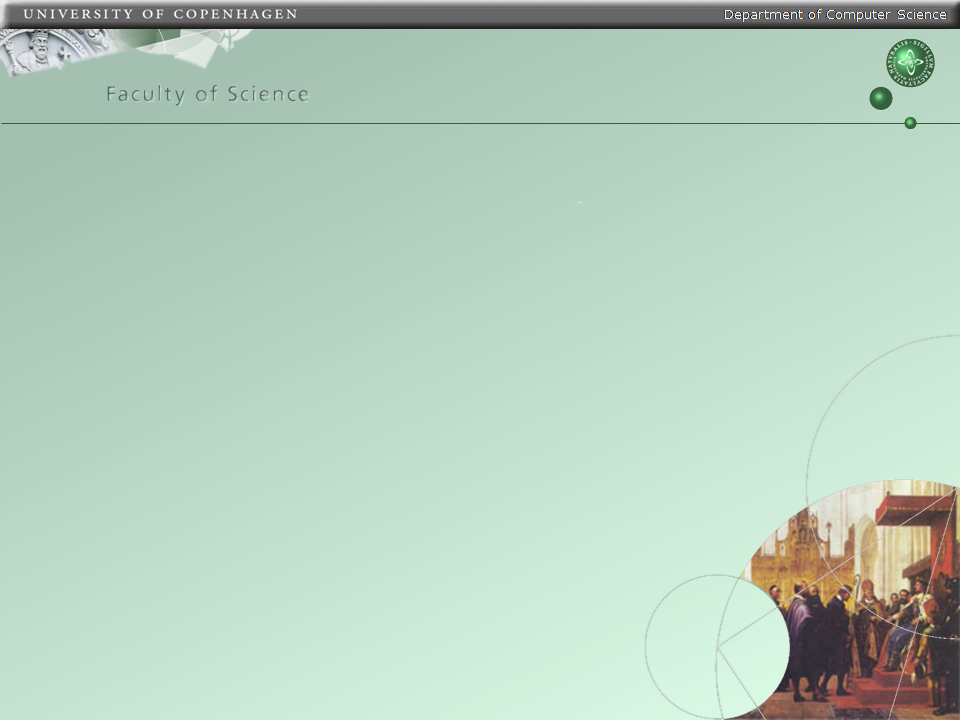
\includegraphics[width=\paperwidth,height=\paperheight]{front}}
{
\begin{frame}[plain]
  \titlepage
\end{frame}
}

% Set background to rest of pages
\usebackgroundtemplate{
\includegraphics[width=\paperwidth,height=\paperheight]{background}}

%
%
%
\begin{frame}
\frametitle{Overview}
\tableofcontents
\end{frame}



%
%
%
\begin{frame}
\frametitle{What is concurrency?}
\section{What is concurrency?}

"Logical control flows are \textit{concurrent} if they overlap in time."
\footnote{\ (BOH, cp. 12)\vspace{2mm}}

\begin{figure}
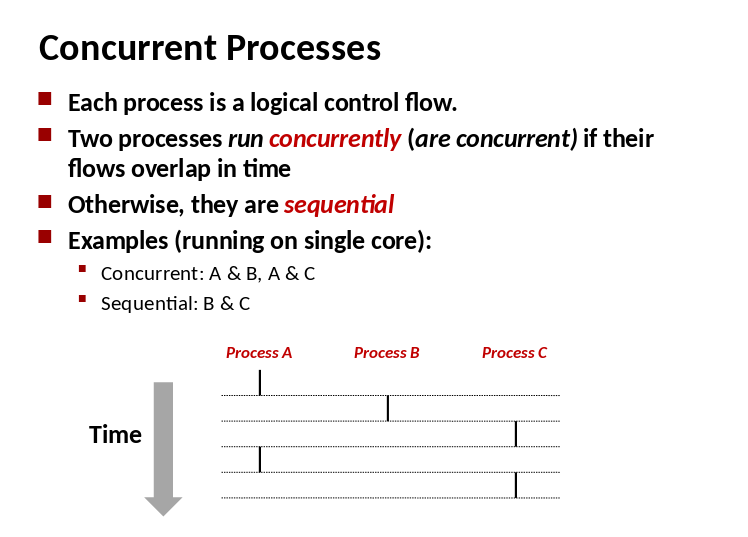
\includegraphics[width=0.8\textwidth]{images/concurrent-processes.png}
\end{figure}
\end{frame}



%
%
%
\begin{frame}
\frametitle{How can we achieve concurrency?}
\section{How can we achieve concurrency?}
We have 3 different set of tools available to use for writing
concurrent programs:\\
\vspace{3mm}
\textbf{Processes}
\begin{itemize}
\item A running program can clone itself into one or more child processes
\item Completely separated memory areas
\end{itemize}
\vspace{2mm}

\textbf{I/O Multiplexing}
\begin{itemize}
\item Resembles event-driven programming
\item I/O operations do not block
\end{itemize}
\vspace{2mm}

\textbf{Threading}
\begin{itemize}
\item Multiple parallel control flows exist within the same process
\item Often the most practical solution
\end{itemize}
\end{frame}



%
%
%
\begin{frame}
\frametitle{Processes}
\subsection{Processes}
How do we use them?

\begin{figure}
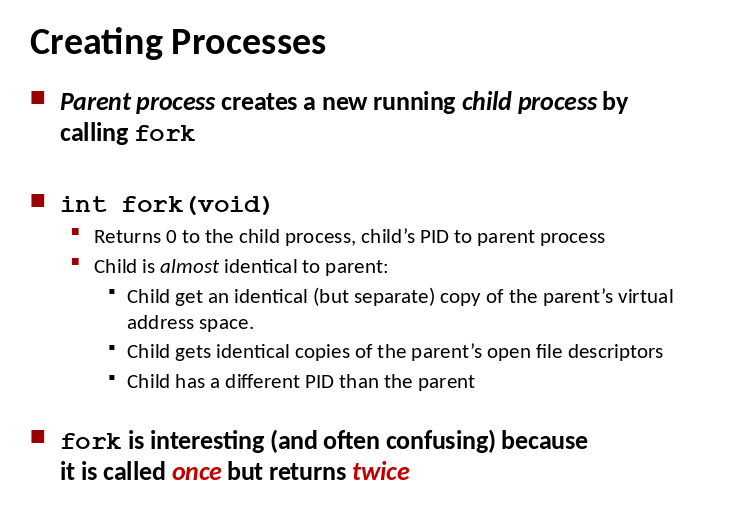
\includegraphics[width=0.8\textwidth]{images/creating-processes.png}
\end{figure}

\end{frame}



%
%
%
\begin{frame}
\frametitle{How to use Processes}

Linux interface for using processes: \texttt{fork}, \texttt{execv}, \texttt{getpid},
\texttt{wait}, \texttt{waitpid}, \texttt{exit}.\\\vspace{3mm}

Concurrency protection mechanisms are not necessary between a process and its child
processes because they operate on completely disjoint memory areas.\\\vspace{3mm}

However, communication between processes is expensive. Common methods are memory
mappings \texttt{(mmap())}, file pipes \texttt{(pipe())}, and sockets.

\end{frame}



%
%
%
\begin{frame}
\frametitle{Processes: Exam question example}
Exam question from re-exam 19/20:

\vspace{-3mm}
\begin{figure}
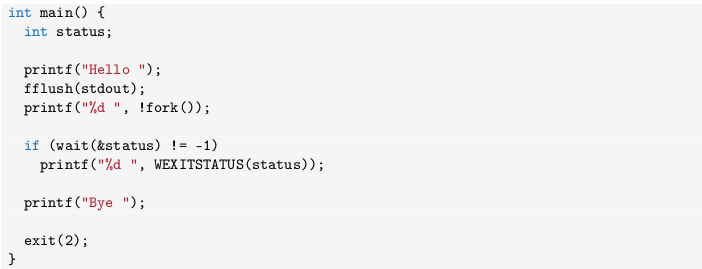
\includegraphics[width=1.0\textwidth]{images/exam_question_1_fork.png}
\end{figure}
\vspace{-3mm}
Which of the following are \textit{possible} valid outputs of the program?
\vspace{2mm}

\begin{columns}
\begin{column}{0.5\textwidth}
\footnotesize
\ \ \ \ \textbf{a)} \texttt{Hello 0 1 Bye 2 Bye}\ \ {\color{OliveGreen}Yes}\\
\ \ \ \ \textbf{b)} \texttt{Hello Bye 1 0 2 Bye}\ \ {\color{red}No}\\
\ \ \ \ \textbf{c)} \texttt{Hello 1 0 Bye 2 Bye}\ \ {\color{OliveGreen}Yes}
\end{column}
\begin{column}{0.5\textwidth}  %%<--- here
\footnotesize
\textbf{d)} \texttt{Hello 1 Bye 0 2 Bye}\ \ {\color{OliveGreen}Yes}\\
\textbf{e)} \texttt{Hello 0 Bye 1 2 Bye}\ \ {\color{red}No}\\
\textbf{f)} \texttt{Hello 0 1 Bye Bye 2}\ \ {\color{red}No}
\end{column}
\end{columns}

\end{frame}



%
%
%
\begin{frame}
\frametitle{I/O Multiplexing}
\subsection{I/O Multiplexing}
I/O operations are blocking. In a webserver \texttt{accept()} blocks control flow
until it receives an incoming connection request.\\\vspace{3mm}

But with I/O Multiplexing we can add a number of file descriptors to a read set,
e.g. \texttt{read-set := \{STDIN\_FILENO, listenfd\}}. This way, a webserver can
read from both without blocking, whenever either is ready for reading.\\\vspace{3mm}

Programming interface: \texttt{select}, \texttt{FD\_ZERO}, \texttt{FD\_CLR},
\texttt{FD\_SET}, \texttt{FD\_ISSET}.\\\vspace{3mm}

Detail: \texttt{select()} is a blocking function.\\
Example in (BOH, sec. 12.2).

\end{frame}



%
%
%
\begin{frame}
\frametitle{Threading}
\subsection{Threading}
Using multiple threads (ie. "multi-threading") is the most common way of achieving
concurrency in programming.\\

\begin{figure}
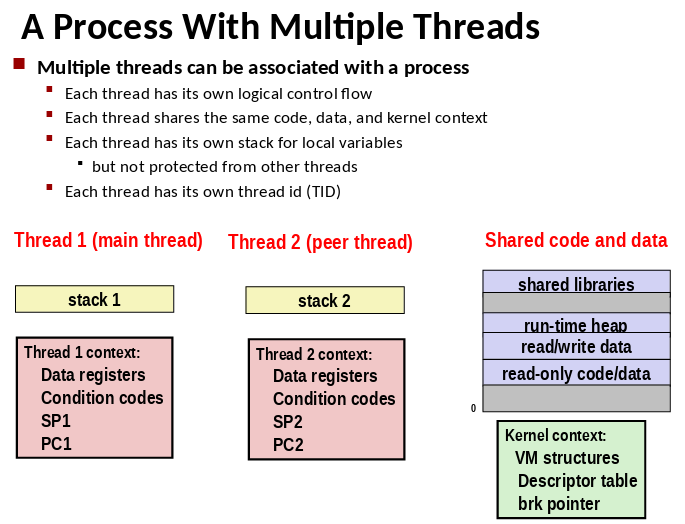
\includegraphics[width=0.8\textwidth]{images/process-with-multiple-threads.png}
\end{figure}

\end{frame}



%
%
%
\begin{frame}
\frametitle{How to use Threads}

Linux (posix) programming interface: \texttt{pthread\_create}, \texttt{pthread\_join},
\texttt{pthread\_detach}, \texttt{pthread\_cancel}, \texttt{pthread\_exit},
\texttt{pthread\_self}, \texttt{pthread\_yield}.\\\vspace{3mm}

Threads are advantageous in many situations because sharing data btw. peer threads
is very easy \texttt{(malloc())}, and overhead for creating threads is significantly
less than for creating processes. Also, compared to I/O Multiplexing, threads are
\textbf{truly} parallel.\\\vspace{3mm}

Threaded programs are exposed to a lot of nasty bugs that can be difficult and
time-consuming to track down.

\end{frame}



%
%
%
\begin{frame}
\frametitle{Data sharing in a threaded program}
Both global and dynamic (malloc'ed) data is shared between threads:

\begin{figure}
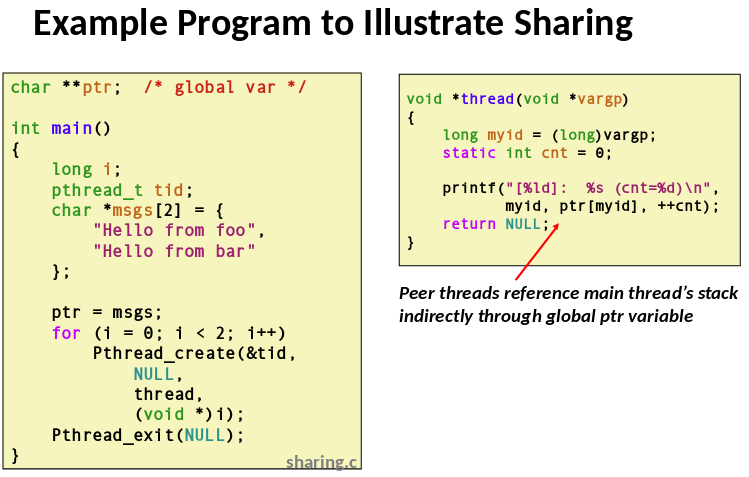
\includegraphics[width=0.9\textwidth]{images/example-program-to-illustrate-sharing.png}
\end{figure}
\end{frame}



%
%
%
\begin{frame}
\section{What can go wrong in concurrent programming}
\frametitle{What can go wrong in concurrent programming}
We will focus only on concurrency issues with multi-threading.\\\vspace{3mm}

\textbf{Common issues}
\begin{itemize}
\item Data races / race conditions
\item Deadlocks
\end{itemize}\vspace{3mm}

\textbf{Other issues that we omit in this lecture}
\begin{itemize}
\item Starvation
\item Contention / congestion
\item Busy-wait loops (extensive resource usage)
\item Priority-inversion
\end{itemize}

\end{frame}



%
%
%
\begin{frame}
\frametitle{Example: What can go wrong (1)}
\begin{figure}
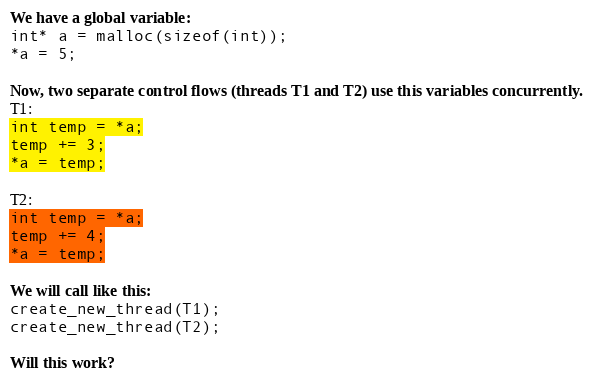
\includegraphics[width=0.9\textwidth]{images/what-can-go-wrong-1.png}
\end{figure}
\end{frame}

\begin{frame}
\frametitle{Example: What can go wrong (2)}
\begin{figure}
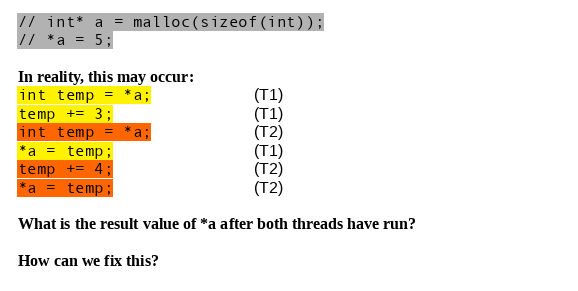
\includegraphics[width=0.9\textwidth]{images/what-can-go-wrong-2.png}
\end{figure}
\end{frame}

\begin{frame}
\frametitle{Example: What can go wrong (3)}
\begin{figure}
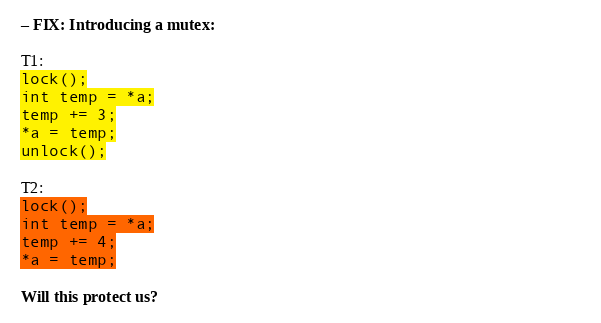
\includegraphics[width=0.9\textwidth]{images/what-can-go-wrong-3.png}
\end{figure}
\end{frame}

\begin{frame}
\frametitle{Example: What can go wrong (4)}
\begin{figure}
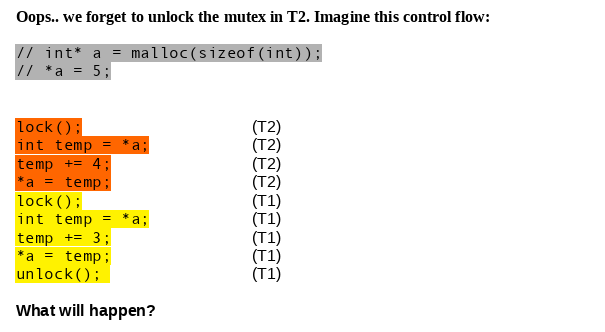
\includegraphics[width=0.9\textwidth]{images/what-can-go-wrong-4.png}
\end{figure}
\end{frame}

\begin{frame}
\frametitle{Example: What can go wrong (5)}
\begin{figure}
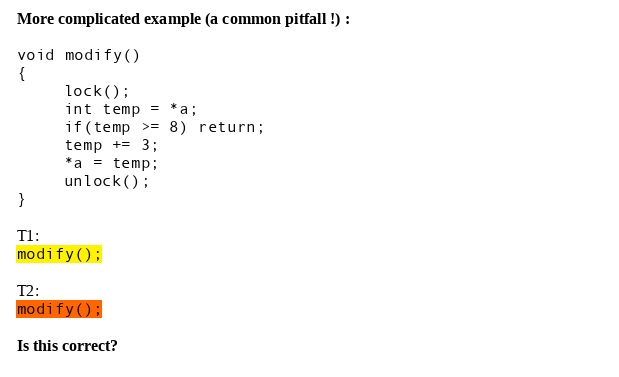
\includegraphics[width=0.9\textwidth]{images/what-can-go-wrong-5.png}
\end{figure}
\end{frame}

\begin{frame}
\frametitle{Example: What can go wrong (6)}
\begin{figure}
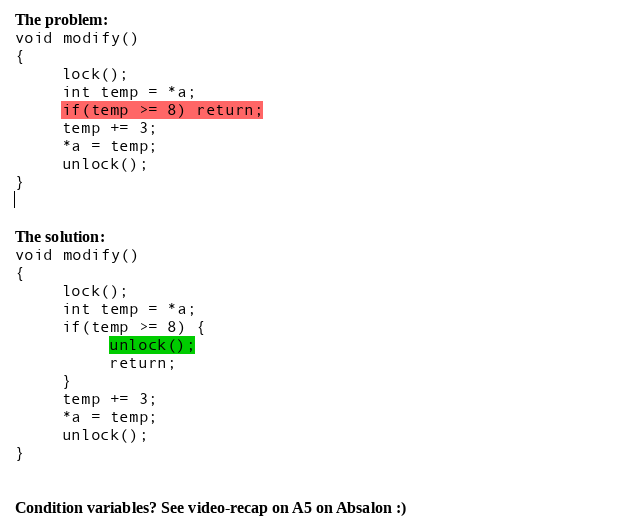
\includegraphics[width=0.85\textwidth]{images/what-can-go-wrong-6.png}
\end{figure}
\end{frame}




%
%
%
\begin{frame}
\section{Concurrency protection mechanisms}
\frametitle{Concurrency protection mechanisms}
Fortunately, we have some powerful tools at our disposal to help us
overcome these issues, provided we use them correctly:\\\vspace{3mm}

\textbf{Mutex}
\begin{itemize}
\item Obtain exclusive access to critical sections
\item \texttt{pthread\_mutex\_(init|destroy|lock|unlock)}
\end{itemize}

\textbf{Condition variable}
\begin{itemize}
\item Threads go to sleep waiting for a specific condition
\item \texttt{pthread\_cond\_(init|destroy|wait|broadcast)}
\end{itemize}

\textbf{Semaphore}
\begin{itemize}
\item Like mutex, except N threads can lock simultaneously
\item \texttt{sem\_init}, \texttt{sem\_destroy}, \texttt{sem\_wait}, \texttt{sem\_post}
\end{itemize}

\end{frame}



%
%
%
\begin{frame}
\frametitle{Processes: Exam question example}
Exam question from re-exam 18/19, covering recap of several OS areas:

\begin{figure}
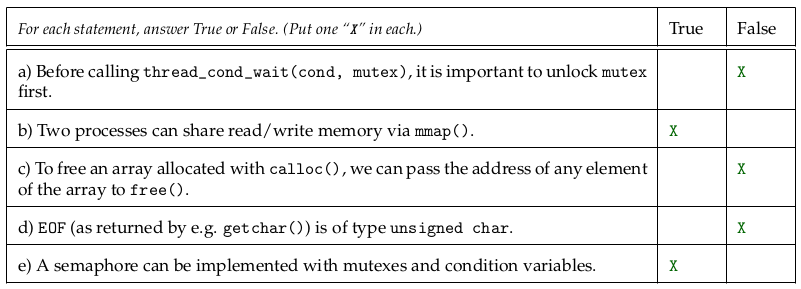
\includegraphics[width=1.0\textwidth]{images/exam_question_2_recap.png}
\end{figure}

\end{frame}



%
%
%
\begin{frame}
\frametitle{Summary}
We have seen how to construct concurrent work flows.

\vspace{5mm}
We have seen what can go wrong in concurrent programming, and how to
fix some common issues.

\vspace{5mm}
We have looked at some exam questions from previous years.

\vspace{5mm}
Good luck in your exam.
\end{frame}



%
%
%
\begin{frame}
\frametitle{Inspirational quote}

\begin{figure}
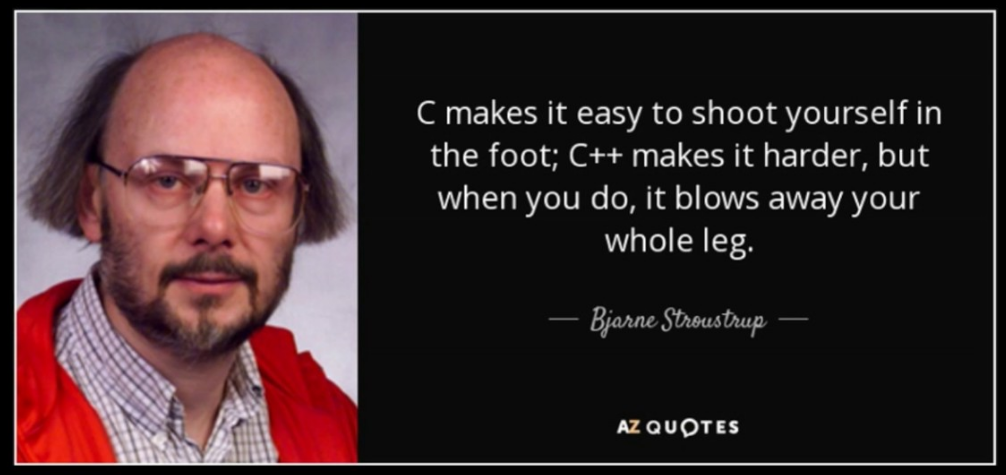
\includegraphics[width=1.0\textwidth]{images/inspirational-quote.png}
\end{figure}

\end{frame}



%
%
%
\begin{frame}
\frametitle{Questions}

???
\end{frame}

\end{document}
